\documentclass{article}
\usepackage{hyperref}
\hypersetup{colorlinks = false, pdfborder = {0 0 0}}
\usepackage[margin=1.3cm]{geometry}
\usepackage{graphicx}
\usepackage{float}
\usepackage{subfig}
\usepackage{multirow}
\setlength\parindent{0pt}

% \begin{reusefigure}[<float spec>]{<ref>}
\newenvironment{reusefigure}[2][htbp]
{\addtocounter{figure}{-1}%
	\renewcommand{\theHfigure}{dupe-fig}% If you're using hyperref
	\renewcommand{\thefigure}{\ref{#2}}% Figure counter is \ref
	\renewcommand{\addcontentsline}[3]{}% Avoid placing figure in LoF
	\begin{figure}[#1]}
	{\end{figure}}

\title{CEGE0023: Offshore and Coastal Engineering\\
Laboratory Report - Wave-flume experiment: wave generation and wave-data analysis}
\author{Alex (Nathalie Alexandra) Tcherdakoff}
\date{SN: 18006289 - Computer Science MEng - SoRA}
\begin{document}
	\maketitle
	\section*{Risk Assessment}
	\begin{figure}[H]
		\centering
		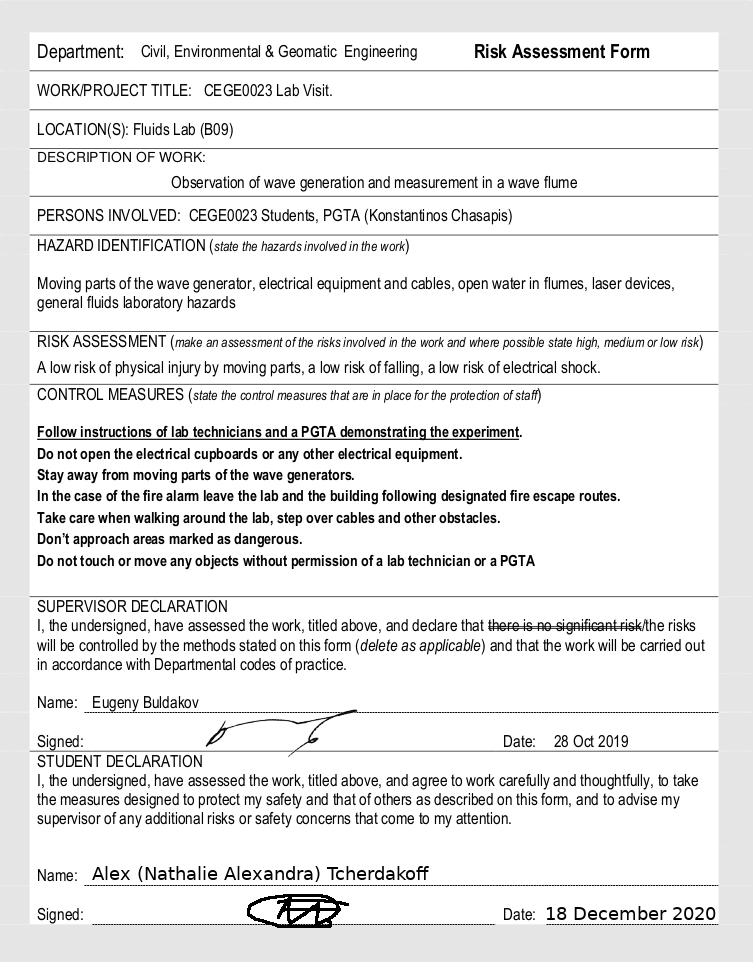
\includegraphics[width=0.745\textwidth]{../graphs/RiskAssessment.png}
		\label{riskassessment}
	\end{figure}
	\section{Abstract}
	This report contains an analysis of the wave-data from recorded waves generated in a laboratory wave-flume experiment. The analysis covers both regular waves (with frequencies $f = 0.5$Hz, 1Hz, and 1.5Hz and respective nominal amplitudes $A = 4$cm, 3cm, and 2cm), as well as random waves (specifically, a 5 minute long sequence simulating a random sea state).
	\section{Experiment Description}
	This experiment is performed in a wave-flume, of which the dimensions are:
	\begin{itemize}
		\item 13m length (working section)
		\item 45cm width
		\item 40cm depth (water height at rest)
	\end{itemize}
	At either end of the wave-flume are piston-type wavemakers: the right-side wavemaker generates the waves, while the left-side wavemaker is to absorb the waves in order to eliminate reflection. However, the wavemaker is more efficient at absorbing long waves; in order to reduce overall reflections and absorb short waves, a horizontal flat metal perforated plate is placed just below water surface, in front of the wave absorber piston. While it is impossible to eliminate all reflections, the aim is to limit them as much as possible to limit experimental error. The wavermakers are connected to a control system, the input to which is the amplitude and frequency of generated regular waves, multiple of which can be superposed in order to create random waves or wave groupings. Wave generation is done using 2 pieces of software: the wave synthesizer designs specific experiments, which can be fed as input to the wave making program, which directly controls the wavemaker movement.\\
	There are 5 wave probes placed throughout the flume in order to measure wave data: these must be calibrated in order to provide a 1 Volt/cm water level change signal to their connected wave monitor. If they are not calibrated properly, this can also lead to experimental error. The data logger then translates the analogue signal from the wave monitor to digital signal, and tranfers the data to the data acquisition software which can both save and inspect the data.\\
	\begin{figure}[H]
		\centering
		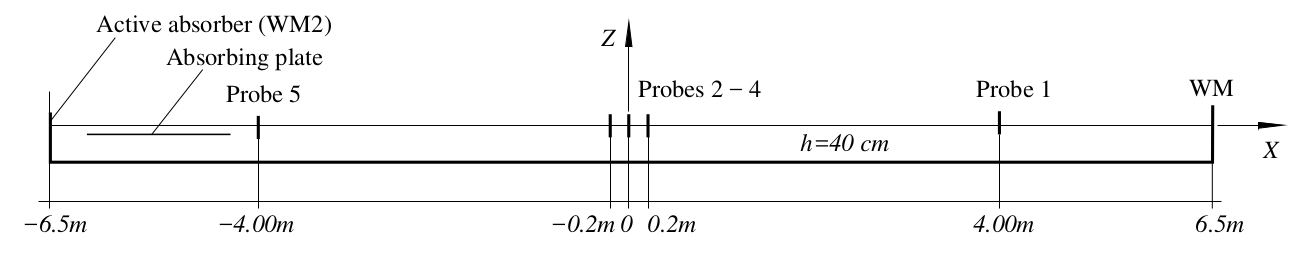
\includegraphics[clip, trim = 0 0.5cm 0 0.5cm,width=0.5\textwidth]{../graphs/experiment.png}
		\caption{Wave flume layout and positions of wave probes \cite{experimentdesc}}
		\label{experiment}
	\end{figure}
	\section{Results}
	\subsection{Regular wave record analysis}
	%Analyse regular wave records for probes 2, 3 and 4. For each wave, measure times between identical phases for different probes. Use the time differences to calculate phase speeds (celerities). Compare calculated phase speeds with theoretical values.\\
	The measured wave data for probes 2, 3, and 4 can be represented using Python \cite{code} (applies to all the graphs in this paper):\\
	\begin{figure}[H]
		\centering
		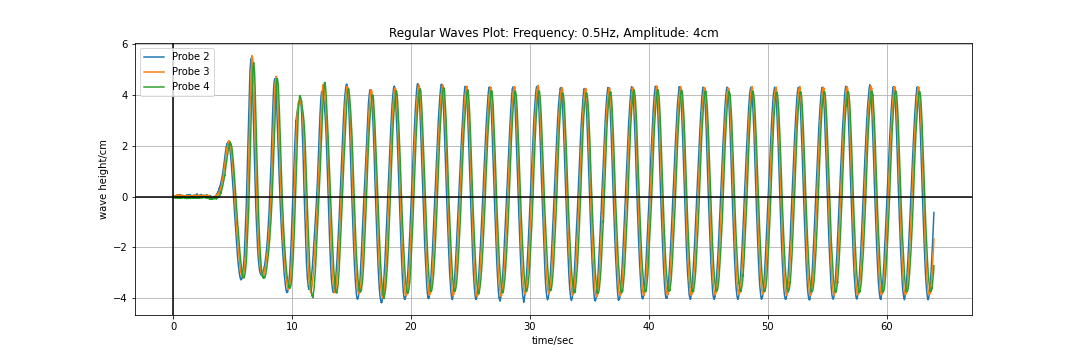
\includegraphics[clip, trim = {3.3cm 0.5cm 3.4cm 1cm},width=\textwidth]{../graphs/F05A4Graph.png}
		\caption{Regular Waves (Frequency = 0.5Hz, Amplitude = 4cm) Profile Representation measured from probes 2 through 4}
		\label{f05a4graph}
	\end{figure}
	\begin{figure}[H]
		\centering
		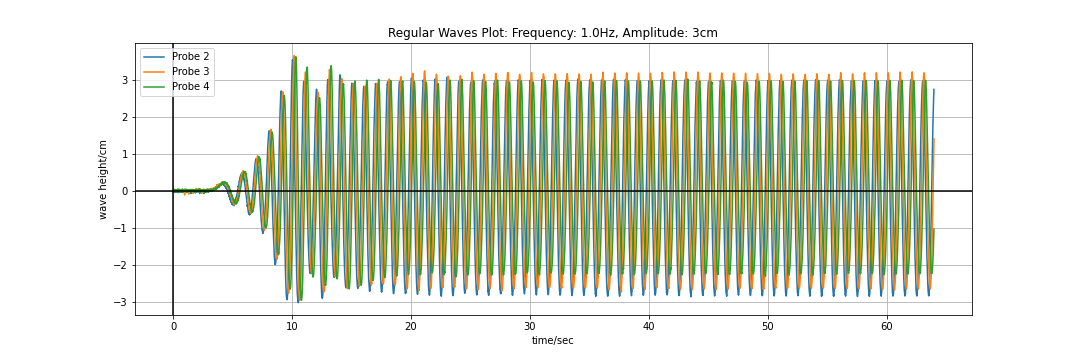
\includegraphics[clip, trim = {3.3cm 0 3.4cm 1cm}, width=\textwidth]{../graphs/F10A3Graph.png}
		\caption{Regular Waves (Frequency = 1.0Hz, Amplitude = 3cm) Profile Representation measured from probes 2 through 4}
		\label{f10a3graph}
	\end{figure}
	\begin{figure}[H]
		\centering
		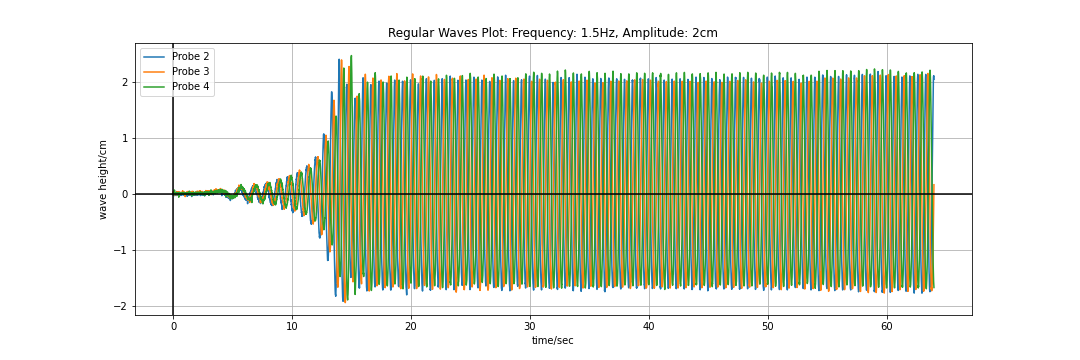
\includegraphics[clip, trim = {3.3cm 0 3.4cm 1cm},width=\textwidth]{../graphs/F15A2Graph.png}
		\caption{Regular Waves (Frequency = 1.5Hz, Amplitude = 2cm) Profile Representation measured from probes 2 through 4}
		\label{f15a2graph}
	\end{figure}
	The previous plots show an overview of the data, including the transitional period at the beginning. In order to analyse the wave record and compare the data, it is more appropriate to graph 1 period (not from the beginning) per record. The following periods were taken from approximately the middle of the records:\\
	\begin{figure}[H]
		\centering
		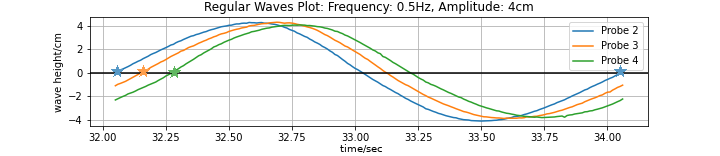
\includegraphics[clip, trim = {1.5cm 0 1.5cm 0},width=\textwidth]{../graphs/F05A4Period.png}
		\caption{Regular Waves (Frequency = 0.5Hz, Amplitude = 4cm) Period Representation measured from probes 2 through 4}
		\label{f05a4period}
	\end{figure}
	\begin{figure}[H]
		\centering
		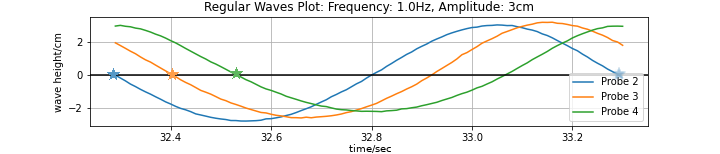
\includegraphics[clip, trim = {1.5cm 0 1.5cm 0}, width=\textwidth]{../graphs/F10A3Period.png}
		\caption{Regular Waves (Frequency = 1.0Hz, Amplitude = 3cm) Period Representation measured from probes 2 through 4}
		\label{f10a3period}
	\end{figure}
	\begin{figure}[H]
		\centering
		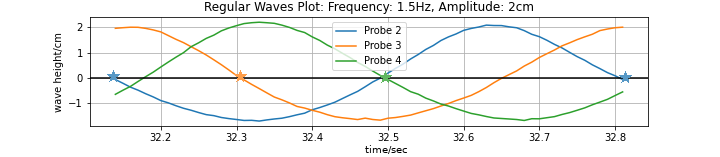
\includegraphics[clip, trim = {1.5cm 0 1.5cm 0},width=\textwidth]{../graphs/F15A2Period.png}
		\caption{Regular Waves (Frequency = 1.5Hz, Amplitude = 2cm) Period Representation measured from probes 2 through 4}
		\label{f15a2}
	\end{figure}
	The following can be calcuated from the data, using the same Python program to measure times between different phases for different probes as was used to generate the previous 3 plots: (theoretical period : $T = 1/f$)\\
	\begin{table}[H]
		\centering
		\begin{tabular}{|c|c|c|c|c|c|}
		\hline
		\multicolumn{3}{|c|}{\textbf{Given Data}} & \multicolumn{3}{c|}{\textbf{Measured Period (determined programmatically)}} \\ \hline
		Wave Frequency & Amplitude & Theoretical Period & Probe 2 & Probe 3 & Probe 4\\ \hline	
		$f = 0.5Hz$ & $A=4cm$ & $T=1/0.5=2.00s$ & $34.06  - 32.05 = 2.01s$ & $34.16 - 32.16 = 2.00s$ & $34.28 - 32.28 = 2.00s$\\ \hline
		$f = 1.0Hz$ & $A=3cm$ & $T=1/1.0=1.00s$ & $33.30 - 32.29 = 1.01s$ & $33.41 - 32.41 = 1.00s$  & $33.57 - 32.57 = 1.00s$\\ \hline
		$f = 1.5Hz$ & $A=2cm$ & $T =1/1.5=0.67s$ & $32.81 - 32.14 = 0.67$ & $32.98 - 32.31 = 0.67s$ & $33.15 - 32.48 = 0.67$\\ \hline
		\end{tabular}
	\caption{Regular Wave Record Analysis: table of results}
	\label{regulartable}
	\end{table}
	The difference between the theoretical and the measured periods is negligible: they are nearly identical. However, now the comparison can be made between the measured celerities: the theoretical celerity can be determined, as in theory the regular waves can be represented as sine waves where the surface elevation $\eta(x,t) = 2\pi A * sin(t/T - x/L)$ and the theoretical celerity $C = L/T$ (the theoretical celerity in Table \ref{celeritytable} was determined using the provided calculator).
	The distance between probes 2 and 4 is 0.4m, this as well as the delay between can be used to calculate the measured celerity: $C_M = 0.4/(P_4 - P_2)$ m/s where $P_2$ and $P_4$ are the starting times of the measured periods from Table \ref{regulartable}.
	\begin{table}[H]
		\centering
		\begin{tabular}{|c|c|c|c|c|}
			\hline
			Wave Frequency & Amplitude & Theoretical Period & \textbf{Theoretical Celerity} & \textbf{Measured Celerity}\\ \hline	
			$f = 0.5Hz$ & $A=4cm$ & $T= 2.00s$ & $C = 1.84747746$ m/s & $C_M = 0.4/(34.28 - 34.06) = 1.81818$ m/s\\ \hline
			$f = 1.0Hz$ & $A=3cm$ & $T=1.00s$ &$C = 1.46373472$ m/s & $C_M = 0.4/(33.57-33.30) = 1.481481$ m/s\\ \hline
			$f = 1.5Hz$ & $A=2cm$ & $T = 0.67s$& $C = 1.04448977$ m/s & $C_M = 0.4/(33.15 - 32.81) = 1.176471$ m/s\\ \hline
		\end{tabular}
		\caption{Regular Wave Record Analysis: table of celerities}
		\label{celeritytable}
	\end{table}
	The measured celerities of the first 2 waves are identical to the theoretical celerity values to $10^{-1}$ degrees of precision. These differences can be attributed to the inevitable experimental errors (coming from refections and probe calibration for example). The 3rd wave's measured and theoretical celerities are more different, only identical to $1$ degree of precision.
	\subsection{Wave length calculation}
	%Use the experimental phase velocities to calculate wave length of each wave. Compare the calculated values with theoretical ones. For each wave determine if it corresponds	to Shallow-water, intermediate-water or deep-water regime.
	Using the measured and theoretical periods and celerities, the measured and theoretical lengths of each wave can be calculated as $L = C*T$ m; these measured and theoretical values can then be compared:\\
	\begin{table}[H]
		\centering
		\begin{tabular}{|c|c|c|c|}
			\hline
			Wave Frequency & Amplitude & \textbf{Theoretical Wave Length $L = C*T$} & \textbf{Measured Wave Length}\\ \hline	
			$f = 0.5Hz$ & $A=4cm$ & $L = 1.84747746 * 2.00 = 3.69495492$ m & $L_M = 1.81818 * 2.00 = 3.63636$ m\\ \hline
			$f = 1.0Hz$ & $A=3cm$ &$L = 1.46373472 * 1.00 = 1.46373472$ m & $L_M = 1.481481 * 1.00 = 1.481481$ m\\ \hline
			$f = 1.5Hz$ & $A=2cm$ & 
			$L = 1.04448977 * 0.67 = 0.699808146$ m & $L_M = 1.176471 * 0.67 = 0.7882356$ m\\ \hline
		\end{tabular}
		\caption{Regular Wave Record Analysis: table of lengths}
		\label{lengthtable}
	\end{table}
	As expected (given the results for the measured celerity), the theoretical and measured values of the first 2 waves are identical to $10^{-2}$ degrees of precision, and the 3rd to $1$ degree. From these results, it can be determined for each wave if it corresponds	to shallow-water, intermediate-water or deep-water regime: given the water depth (\ref{experiment}) $d = 40$cm or $d = 0.40$ m, and that:
	\begin{itemize}
		\item shallow water: $d/L < 1/25$
		\item transitional water: $1/25 < d/L < 1/2$
		\item deep water:  $d/L > 1/2$
	\end{itemize} 
	\begin{table}[H]
		\centering
		\begin{tabular}{|c|c|c|c|}
			\hline
			Wave Frequency & Amplitude & $d/L$ & \textbf{Depth}\\ \hline	
			$f = 0.5Hz$ & $A=4cm$ & $0.40/3.69495492 = 0.1082557$& $0.04 < 0.1082557 < 0.5$ : intermediate water\\ \hline
			$f = 1.0Hz$ & $A=3cm$ &$0.40/ 1.46373472 = 0.27327356$ & $0.04 < 0.27327356 < 0.5$ : intermediate water\\ \hline
			$f = 1.5Hz$ & $A=2cm$ & 
			$0.40 / 0.699808146 = 0.57158522$ & $0.57158522 > 0.5$ : deep water\\ \hline
		\end{tabular}
		\caption{Regular Wave Record Analysis: table of depths}
		\label{depthtable}
	\end{table}
	The 3rd wave being in the deep-water regime is possibly the reason the measured and theoretical values of wave-length and celerity are more different than for the other 2 waves.
	\subsection{Celerity and wave length: theoretical relationship}
	%Plot a graph demonstrating the theoretical relationship between celerity and wave length. Use non-dimensional	values. Scale the wave speed by the shallow wave celerity ($C_s = sqrt(gh)$) and the wave length by the water depth. Place experimental	data points to the same graph. If necessary, refer to the graph in previous discussion.
	\begin{figure}[H]
		\centering
		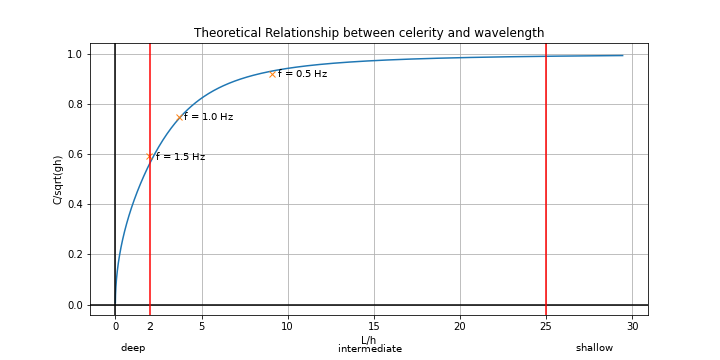
\includegraphics[width=\textwidth]{../graphs/celerityvslength.png}
		\caption{Theoretical relationship between celerity and wave length}
		\label{celerityvslength}
	\end{figure}
	\subsection{Measured vs. theoretical waves}
	%Select a single wave period from probe 3 records of each regular wave (from one zero-crossing to another). Calculate the actual wave height, compare it with the nominal	wave height. Plot the selected period of each wave in the same graph. Scale surface elevation by the measured wave amplitude (a = H/2) and time by the wave period. Apply a suitable time shift to have same phases for all wave plots. In the same graph plot a sinusoidal wave with a = 1. Compare the shapes of the measured and theoretical waves. Indicate up to 3 reasons why the shapes of the measured waves are different from the theoretical one.
	Using 1 wave period measured by probe 3 for each wave, the wave height can be calculated and compared to the nominal wave height: 
	\begin{figure}[H]
		\centering
		\subfloat{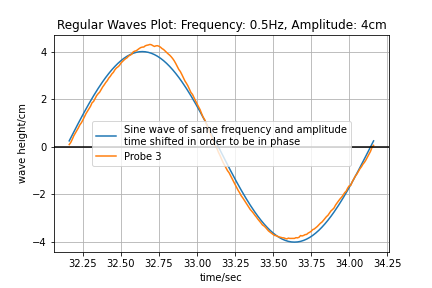
\includegraphics[clip,trim={.2cm 0 1cm 0},width=0.33 \textwidth]{../graphs/F05A4Probe3.png}}
		\subfloat{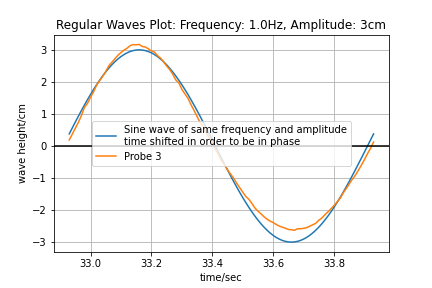
\includegraphics[clip,trim={.2cm 0 1cm 0},width=0.33 \textwidth]{../graphs/F10A3Probe3.png}}
		\subfloat{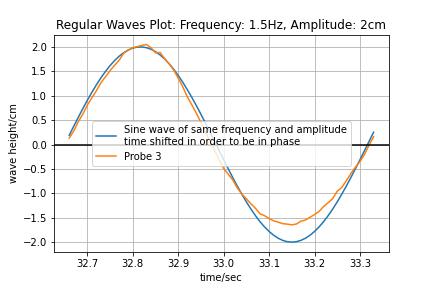
\includegraphics[clip,trim={.2cm 0 1cm 0},width=0.33 \textwidth]{../graphs/F15A2Probe3.png}}
		\caption{Regular Wave Periods measured by Probe 3 compared to sine wave (frequencies f = 0.5 Hz, 1.0 Hz, and 1.5 Hz respectively, from left to right)}
		\label{individualperiods}
	\end{figure}
	For all of the experimental waves, probe 3 measures a higher peak and trough than the expected sinusoidal wave; this can be observed in the following plot with scaled values, and the wave periods overlaid:\\
	\begin{figure}[H]
		\centering
		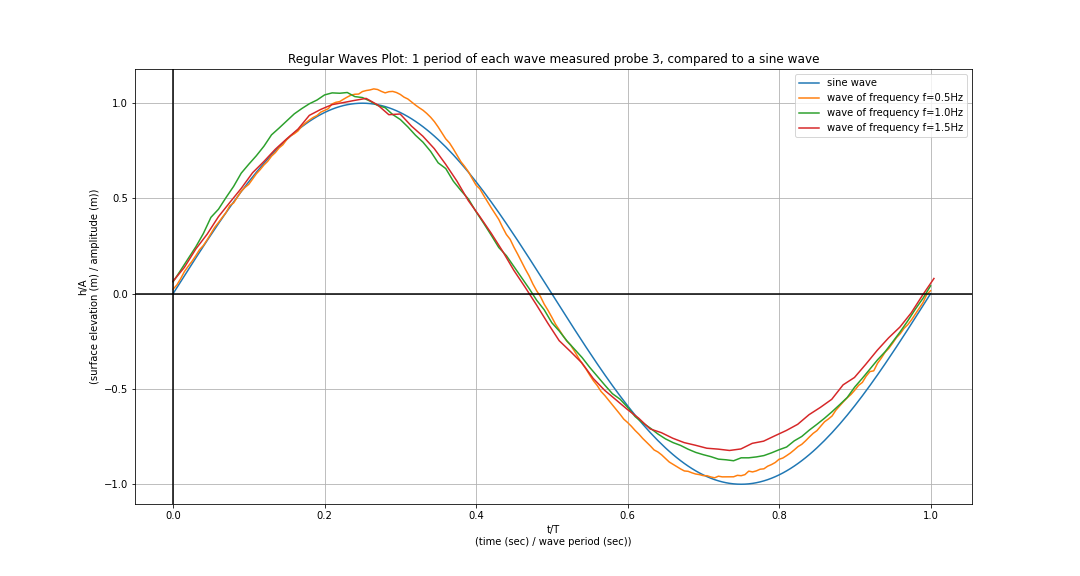
\includegraphics[clip, trim = {2cm 1cm 2cm 1cm},width=\textwidth]{../graphs/Probe3.png}
		\caption{Single wave period measured by probe 3 for each experimental wave, scaled and compared to a sine wave}
		\label{probe3}
	\end{figure}
	The higher peaks and shallower troughs as well as assymetry of the wave shapes in the experimental wave data measured by probe 3 can be explained by the unavoidable experimental errors (such as probe calibration errors, reflections due to wave absorption being imperfect), and a mismatch between the linear wave generation and the nonlinear nature of the experimental components.
	\subsection{Wave amplitude variations}
	%Analyse developed periodic wave records for all probes. Are wave amplitudes constant in space and time? Indicate up to 3 reasons of amplitude variations.
	\begin{figure}[H]
		\centering
		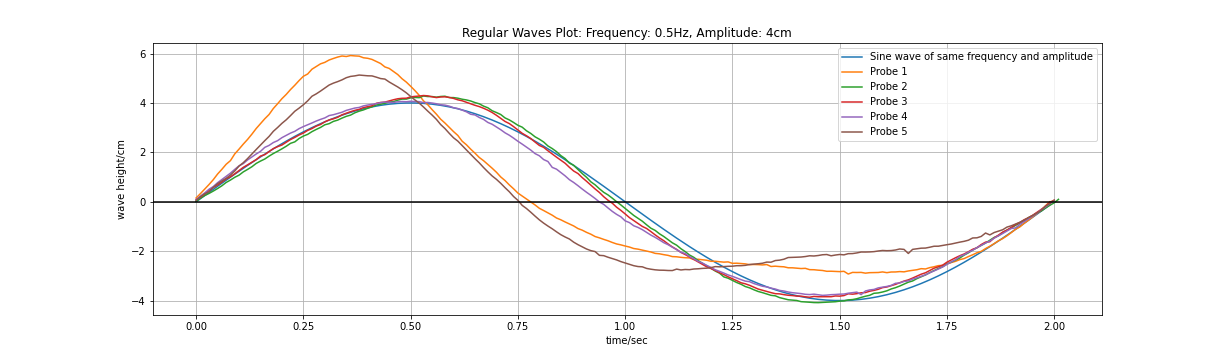
\includegraphics[clip, trim = {3.3cm 0.5cm 3.4cm 1cm},width=\textwidth]{../graphs/F05A4AllProbes.png}
		\caption{Regular Waves (Frequency = 0.5Hz, Amplitude = 4cm): time-shifted period-comparison of all probes and a sine wave}
		\label{f05a4allprobes}
	\end{figure}
	\vspace{-.5cm}
	\begin{figure}[H]
		\centering
		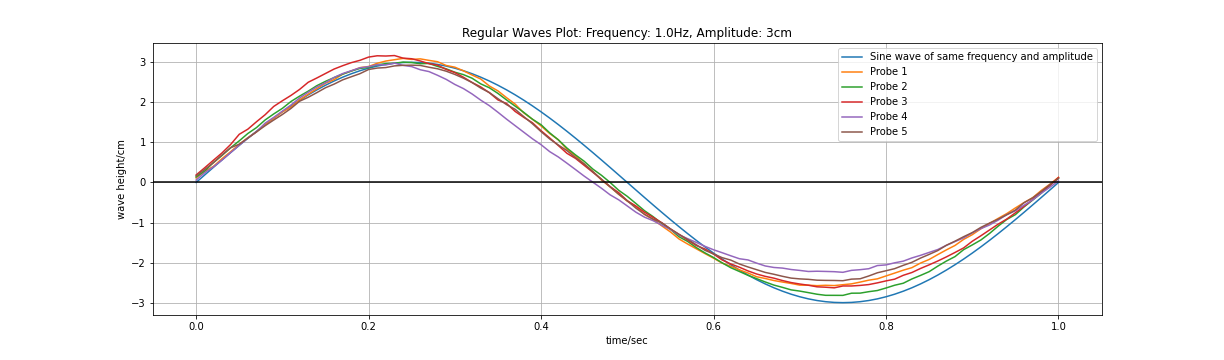
\includegraphics[clip, trim = {3.3cm 0.5cm 3.4cm 1cm},width=\textwidth]{../graphs/F10A3AllProbes.png}
		\caption{Regular Waves (Frequency = 1.0Hz, Amplitude = 3cm): time-shifted period-comparison of all probes and a sine wave}
		\label{f10a3allprobes}
	\end{figure}
	\vspace{-.5cm}
	\begin{figure}[H]
		\centering
		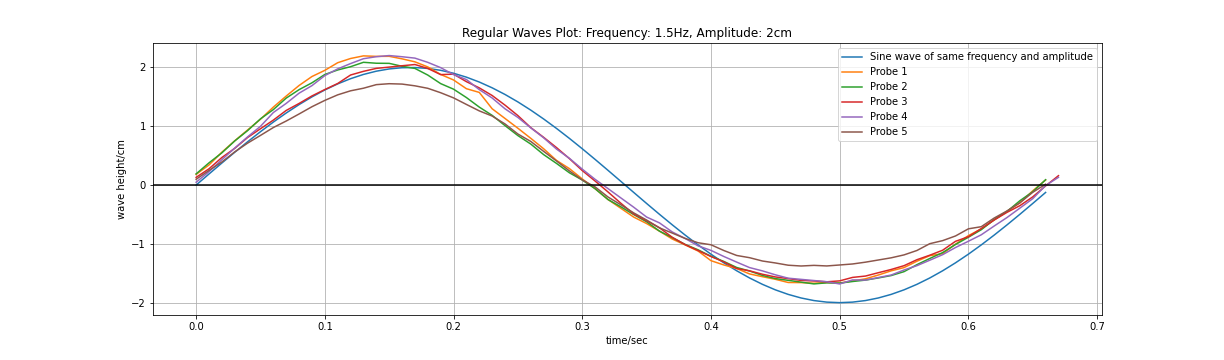
\includegraphics[clip, trim = {3.3cm 0.5cm 3.4cm 1cm},width=\textwidth]{../graphs/F15A2AllProbes.png}
		\caption{Regular Waves (Frequency = 1.5Hz, Amplitude = 2cm): time-shifted period-comparison of all probes and a sine wave}
		\label{f15a2allprobes}
	\end{figure}
	The previous Figures \ref{f05a4allprobes}, \ref{f10a3allprobes}, and \ref{f15a2allprobes} show analyses of developed periodic wave records for all probes compared to each other and to a regular sine wave of the same freqency and amplitude. These graphs show that the wave amplitudes are indeed \textbf{not} constant in space or time, as probes 1 and 5 for the 1st wave show higher peaks and shallower troughs than the rest of the probes as well as the sine wave, for example, and probe 5 for the 3rd waves shows overall lower peaks as well as shallower troughs. The inconsistencies with the first and last probes can be associated with the probes' proximity to the 2 wavemakers, and overall amplitude inconsistencies in the experiment can also be associated with experimental error (such as wave probe calibration imperfection, residual wave reflections, etc..) as well as, again, the mismatch between the linear wave generation, and the non-linear nature of the waves (assymetry in wave shape also leads to different wave amplitudes at different locations).
	\subsection{Wave front evolution}
	%Analyse the wave front evolution recorded by probes 1 and 5. Compare the times when the wave height at the location of each probe growth to a small value (say 5\% of the height of a developed regular wave). 2 Use the time difference to calculate the speed of the wave front for different wave frequencies. Compare it with the theoretical	values of celerity, group velocity and shallow water celerity.
	The wave front evolution can be analysed using probes 1 and 5's recordings for all the waves, specifically observing the beginning of the waves. The peaks and troughs of the values are encompassed by envelopes:\\
	\begin{figure}[H]
		\centering
		\subfloat{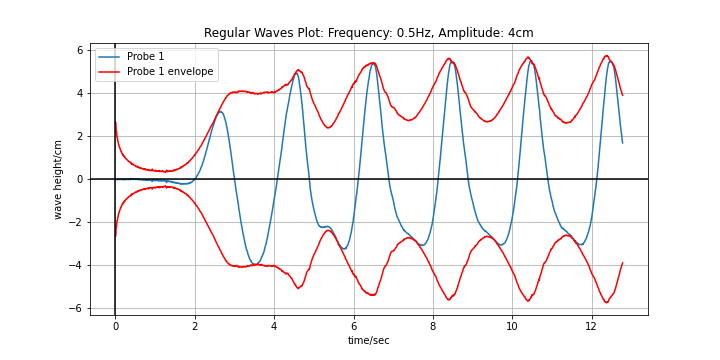
\includegraphics[clip,trim={1.5cm 0.5cm 2cm 0.8cm},width=0.5 \textwidth]{../graphs/F05A4Probe1Envelope.png}}
		\subfloat{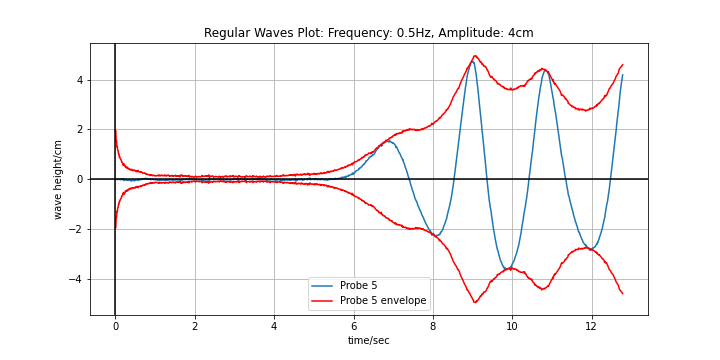
\includegraphics[clip,trim={1.5cm 0.5cm 2cm 0.8cm},width=0.5 \textwidth]{../graphs/F05A4Probe5Envelope.png}}
		\caption{Wave Front Evolution for wave of frequency f = 0.5 Hz as measured by Probe 1 and 5 with wave envelopes}
		\label{wave1envelope}
	\end{figure}
	\vspace{-.5cm}
	\begin{figure}[H]
		\centering
		\subfloat{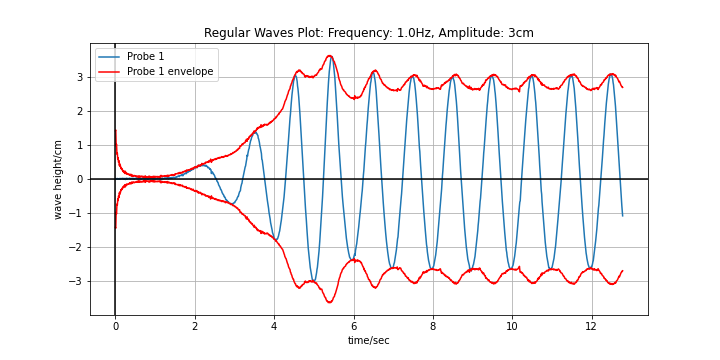
\includegraphics[clip,trim={1.5cm 0.5cm 2cm 0.8cm},width=0.5 \textwidth]{../graphs/F10A3Probe1Envelope.png}}
		\subfloat{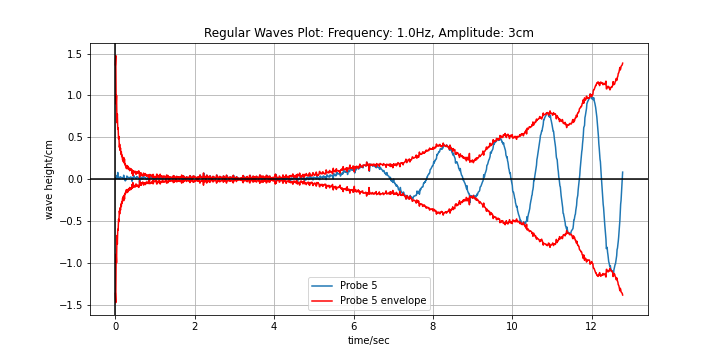
\includegraphics[clip,trim={1.5cm 0.5cm 2cm 0.8cm},width=0.5 \textwidth]{../graphs/F10A3Probe5Envelope.png}}
		\caption{Wave Front Evolution for wave of frequency f = 1.0 Hz as measured by Probe 1 and 5 with wave envelopes}
		\label{wave2envelope}
	\end{figure}
	\vspace{-.5cm}
	\begin{figure}[H]
		\centering
		\subfloat{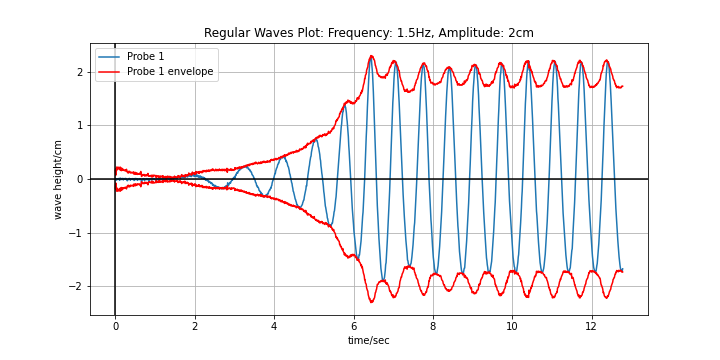
\includegraphics[clip,trim={1.5cm 0.5cm 2cm 0.8cm},width=0.5 \textwidth]{../graphs/F15A2Probe1Envelope.png}}
		\subfloat{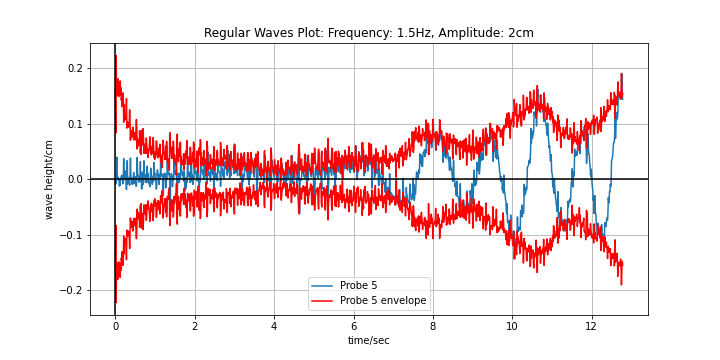
\includegraphics[clip,trim={1.5cm 0.5cm 2cm 0.8cm},width=0.5 \textwidth]{../graphs/F15A2Probe5Envelope.png}}
		\caption{Wave Front Evolution for wave of frequency f = 1.5 Hz as measured by Probe 1 and 5 with wave envelopes}
		\label{wave3envelope}
	\end{figure}
	These envelopes can then be directly compared to each other (as seen in Figures \ref{f05a4envelopes}, \ref{f10a3envelopes}, and \ref{f15a2envelopes}):\\
	\begin{figure}[H]
		\centering
		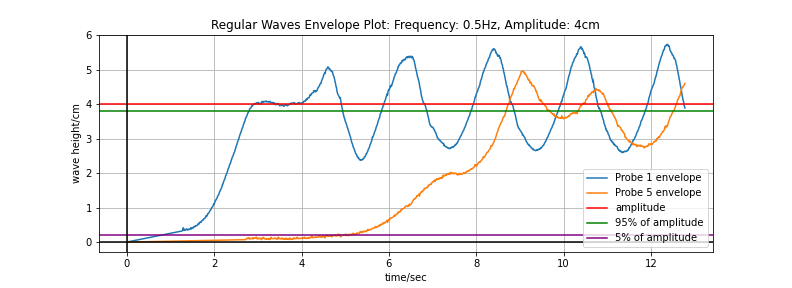
\includegraphics[clip, trim = {1cm 0.1cm 1cm 0.5cm},width=\textwidth]{../graphs/F05A4Probes1and5Envelope.png}
		\caption{Regular Waves (Frequency = 0.5Hz, Amplitude = 4cm): Probes 1 and 5 envelopes comparison}
		\label{f05a4envelopes}
	\end{figure}
	\vspace{-.5cm}
	\begin{figure}[H]
		\centering
		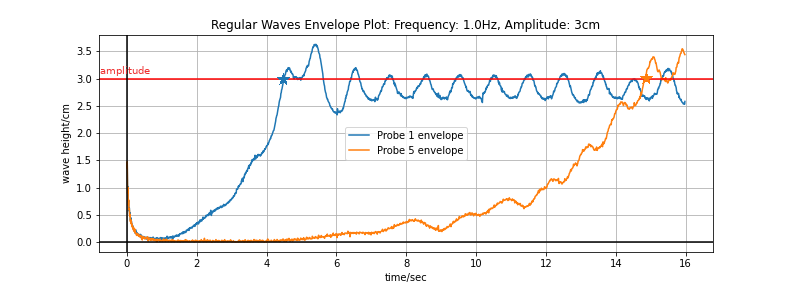
\includegraphics[clip, trim = {1cm 0.1cm 1cm 0.5cm},width=\textwidth]{../graphs/F10A3Probes1and5Envelope.png}
		\caption{Regular Waves (Frequency = 1.0Hz, Amplitude = 3cm): Probes 1 and 5 envelopes comparison}
		\label{f10a3envelopes}
	\end{figure}
	\vspace{-.5cm}
	\begin{figure}[H]
		\centering
		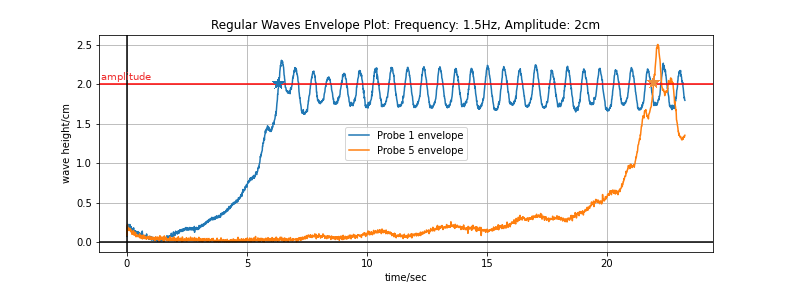
\includegraphics[clip, trim = {1cm 0.1cm 1cm 0.5cm},width=\textwidth]{../graphs/F15A2Probes1and5Envelope.png}
		\caption{Regular Waves (Frequency = 1.5Hz, Amplitude = 2cm): Probes 1 and 5 envelopes comparison}
		\label{f15a2envelopes}
	\end{figure}
	For Figures \ref{f05a4envelopes}, \ref{f10a3envelopes}, and \ref{f15a2envelopes}, the wave height at the location of each probe grew to a small value (at 5\% of the height of a developed regular wave) is identified by the blue and orange curves crossing the purple line (the exact values determined programatically \cite{code}). There are 8m between probes and 5 \ref{experiment}, so $C_M = 8/(P_5 - P_1)$ where $P_5$ and $P_1$ are the probe 5 and 1 crossings, respectively. The values calculated for theoretical celerity $C$ in previous sections still hold. 
	5\% of each of these waves' amplitudes qualifies as shallow water, therefore the group velocity $C_g$ for all these waves is  the same as shallow water celerity $C_s = \sqrt{gh} = \sqrt{9.80665 * 0.40} = 1.98057$ m/s for all waves.\\
	The following values in Table \ref{smallwavefronttable} can therefore be derived in order to compare them:\\
	\begin{table}[H]
		\centering
		\begin{tabular}{|c|c|c|c|c|c|}
			\hline
			Amplitude & \textbf{$P_1$} & \textbf{$P_5$} & \textbf{Measured Celerity} & Theoretical Celerity & Group Velocity  = Shallow Water Celerity\\ \hline
			$A = 4$ cm & 0.78s & 4.67s & $C_M = 2.05655527$ m/s & $C = 1.84747746$ m/s & {\multirow{3}{*}{$C_g = C_s = 1.98057$ m/s}}\\ \cline{1-5}
			$A = 3$ cm & 1.51s & 5.91s & $C_M = 1.81818182$ m/s & $C = 1.4637472$ m/s & {} \\ \cline{1-5}
			$A = 2$ cm & 1.85s & 7.83s & $C_M = 1.33779264$ m/s & $C = 1.04448977$ m/s & {} \\ \hline
		\end{tabular}
	\caption{Table of celerity calculations: probes 1 and 5 first recording of 5\% of the wave amplitude}
	\label{smallwavefronttable}
	\end{table}
	For the first 2 waves, the measured celerities are closest to the group velocity (or the shallow-water celerity), whereas for the third wave, the measured celerity is nearest to the theoretical celerity (this could be due to experimental error, or partially to the fact that out of the 3 sets of waves, the 3rd one corresponds to a deeper-water regime).
	\subsection{Different speeds of energy propagation in the wave front}
	%Repeat the previous analysis using times when wave heights at the probes positions	almost reach the height of a developed wave (say 95\%). Calculate the corresponding velocity for each wave. Compare it with the theoretical values of celerity, group velocity and shallow water celerity. Why do you observe different speeds of energy propagation in the wave front?
	For Figures \ref{f05a4envelopes}, \ref{f10a3envelopes}, and \ref{f15a2envelopes}, the wave height at the location of each probe grew to a large value (at 95\% of the height of a developed regular wave) is identified by the blue and orange curves crossing the green line (the exact values determined programatically \cite{code}). The values for measured celerity, theoretical celerity, and shallow water celerity from the previous section still hold. However, the waves here are not shallow, they are of the depth-regime previously specified: the first 2 waves qualified previously as transitional water and the 3rd wave as deep water. Therefore, the group velocity  $C_g$ for the first 2 waves is :
	\begin{itemize}
		\item \( \displaystyle C_g = \frac{1 + \frac{4\pi h/L}{sinh(4\pi h/L)}}{2} * C \) for the first 2 waves (using the previously calculated theoretical wavelengths)
		\begin{list}{$\circ$}{}
			\item \( \displaystyle C_g = \frac{1 + \frac{4\pi 0.40/3.69495492}{sinh(4\pi 0.40/3.69495492)}}{2} * C = 0.873617 * C = 1.61398772\) m/s for wave 1
			\item \( \displaystyle C_g = \frac{1 + \frac{4\pi 0.40/}{sinh(4\pi 0.40/1.46373472)}}{2} * C = 0.610884 * C = 0.894179745\) m/s for wave 2
		\end{list}
		\item $C_g = \frac{C}{2} = 0.522244885$ m/s for the 3rd wave
	\end{itemize} The following values in Table \ref{largewavefronttable} can therefore be derived:\\
	\begin{table}[H]
		\centering
		\begin{tabular}{|c|c|c|c|c|c|c|}
			\hline
			Amplitude & \textbf{$P_1$} & \textbf{$P_5$} & \textbf{Measured Celerity} & Theoretical Celerity & Group Velocity & Shallow Water Celerity\\ \hline
			$A = 4$ cm & 2.8s & 8.68s & $C_M = 1.36054422$ m/s & $C = 1.84747746$ m/s & $C_g = 1.61398772$ m/s &{\multirow{3}{*}{$C_s = 1.98057$ m/s}}\\ \cline{1-6}
			$A = 3$ cm & 4.46s & 14.78s & $C_M = 0.775193799$ m/s & $C = 1.4637472$ m/s & $C_g = 0.894179745$ m/s & {}\\ \cline{1-6}
			$A = 2$ cm & 6.3s & 21.92s & $C_M = 0.512163893$ m/s & $C = 1.04448977$ m/s & $C_g = 0.522244885$ m/s & {} \\ \hline
		\end{tabular}
		\caption{Table of celerity calculations: probes 1 and 5 first recording of 95\% of the wave amplitude}
		\label{largewavefronttable}
	\end{table}
	Here, all the measured celerities are nearest in value to the group velocity.\\
	Different speeds of energy propagation in the wave front are observed as the more reliable of all the theoretical celerities was shown here to be the one that fluctuates depending on the depth regime of the water observed: the group velocity. Reasons for this include probes 1 and 5's proximities to the wavemakers performing opposing actions (and the absorbing plate), as well as the mismatch between the nonlinear nature of the waves and the supposedly linear wave generation, and finally, experimental errors. Certain fluctuations are also more likely to have inaccuracies, as the absorbing mechanism is more effective at reducing the longer waves: shorter waves are therefore more likely to be counteracted by unabsorbed reflections, possibly explaining the 3rd wave's measured celerity in the previous section. 
	\subsection{Random wave record analysis}
	%Analyse a random wave record for probe 3. Calculate the significant wave height	($H_s$) and the mean zero-crossing period ($T_z$) of this wave sequence.
	\begin{figure}[H]
		\centering
		\subfloat{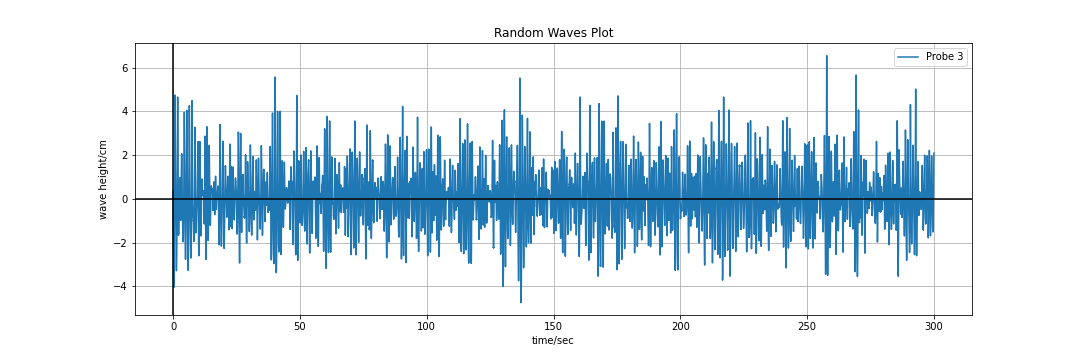
\includegraphics[clip, trim = {3cm 0.2cm 3cm 1cm},width=\textwidth]{../graphs/Rand1thGraph.png}}
		\\
		\subfloat{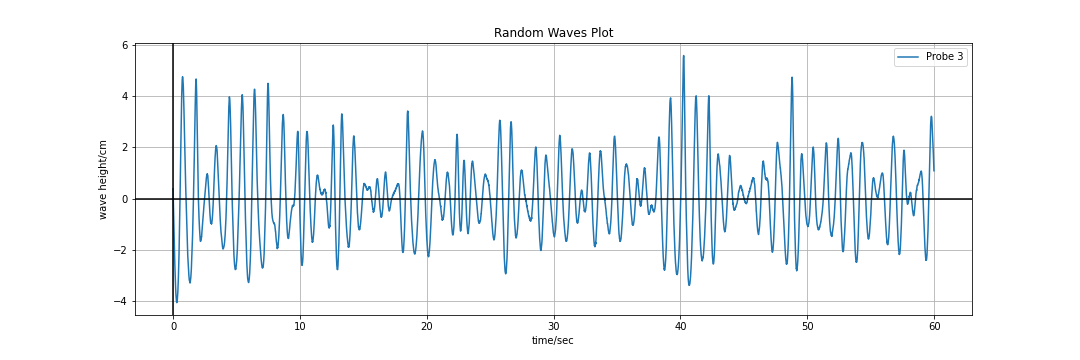
\includegraphics[clip, trim = {3cm 0.2cm 3cm 1cm},width=\textwidth]{../graphs/Rand5thGraph.png}}\\
		\subfloat{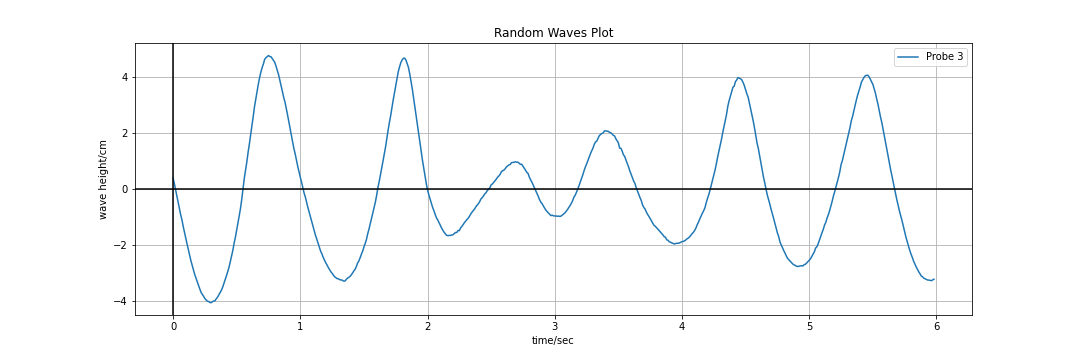
\includegraphics[clip, trim = {3cm 0.2cm 3cm 1cm},width=\textwidth]{../graphs/Rand50thGraph.png}}
		\caption{Random Sea State: randomly generated waves - analysis at different scales}
		\label{randomgraph}
	\end{figure}
	Each period and height in the random wave sequence represented in Figure \ref{randomgraph} was collected programatically, from which the root mean square wave height $H_{RMS}$, the significant wave height $H_s$ and the mean zero-crossing period $T_z = T_0$ have been computed using the following formulae where N is the number of periods in the record, total:
	\begin{itemize}
		\item \( \displaystyle H_{RMS} = (\frac{1}{2}\sum_{i = 1}^{N}H_i^2)^{1/2} = \) \textbf{4.199038328054618 cm}
		\item \( \displaystyle H_s=\sqrt{2} H_{RMS} =\) \textbf{5.938336952459287 cm}
		\item \( \displaystyle T_0 = \frac{1}{N}\sum_{i = 1}^{N} T_{0,i} =\) \textbf{0.8984638554216868 s}
	\end{itemize}
	\subsection{Maximum wave height for 3 hour storm at project site}
	Use Froude similarity law to scale the random wave experimental data to full-scale	conditions of your Design Project site. Calculate the corresponding values of $H_s$, $T_z$ and the duration of the wave sequence. Assuming Rayleigh distribution, find	expected maximum wave height for a 3 hours storm at your project site. Comment on the applicability of Rayleigh distribution.
	\section{Conclusions}
	\begin{thebibliography}{1}
		\bibitem{experimentdesc} Wave generation in a wave-flume experiment and analysis of experimental wave data - Experiment Description and Report Assignment
		\bibitem{code} Github Repository by user Nathalex (Nathalie Alexandra "Alex" Tcherdakoff)\\ \href{https://github.com/nathalex/Wave-Flume-Lab-Report}{\textbf{\textit{https://github.com/nathalex/Wave-Flume-Lab-Report}}}
	\end{thebibliography}
\end{document}